
\documentclass[apj]{emulateapj}

\usepackage{graphicx}
\usepackage{amssymb}
\usepackage{amsmath}
\usepackage{natbib}
\bibliographystyle{apj}
\usepackage[breaklinks,colorlinks,citecolor=blue,linkcolor=magenta]{hyperref}
\shorttitle{Short Title}
\shortauthors{Zhou et al.}

%%% new command %%%
\newcommand{\ima}{\texttt{ima} files }
\newcommand{\flt}{\texttt{flt} files }
\newcommand{\eps}{$\mathrm{e}^{-}/\mathrm{s}$}
\begin{document}
\title{Variability of Planetary Mass Companion 2M1207 B}
\shorttitle{Variability of 2M1207 B}
\author{Yifan Zhou, Daniel Apai, Glenn Schneider, ...}
\affil{The University of Arizona}

\begin{abstract} Rotational modulations in disk-integrated light of
brown dwarfs have recently provided powerful constraints on the
properties of ultracool atmospheres, including longitudinal and
vertical cloud structures and cloud evolution. Furthermore, detection
of periodic light curve variations can directly probe the rotational
periods of ultracool objects.

We present here, for the first time, time-resolved high-precision
photometric measurements of a planetary-mass companion, 2MASS1207b, to
a brown dwarf primary. Using HST/WFC3 and point spread function %in
combination with two spacecraft roll angles we detect photometric
modulations in the light curve. The amplitude is XXX\% in the F160W
and XXX\% in the F125W filters; we find a consistent period and
similar phase in both bands. Joint fit to the lightcurve in both bands
suggest a period of XX$\pm$XXh. The relative amplitudes in the two
filters are very similar to that found in a recent study of a field
(high-gravity) L-dwarf, suggesting that the cloud structures that
introduce the photometric modulations are similar in high- and
low-gravity objects. Importantly, our study also measures, for the
first time, the rotational period for directly imaged planetary-mass
companion.
\end{abstract}

\keywords{kw1, kw2, ...}
\maketitle
%
\section{Introduction}

Cloud properties in high- and low-gravity objects -- thick clouds: an
explanation for very red and faint near-infrared fluxes of directly
imaged planets

Rotational mapping is powerful: successes in brown dwarfs...

The target 2M1207b... contrast The key challenge of obtaining the
lightcurve of 2M1207b is the high contrast to and small separation
from 2M1207A.


In this Letter we present the first high-contrast, high-precision,
time-resolved observations of a directly imaged planet or
planetary-mass object. We successfully detect rotational modulation
and measure the amplitudes in two bands and determine the rotational
period.

\section{Observation} We obtained direct images of the 2M1207A+b
system on UT 2014 April 11 {\bf give full time stamp} using the Hubble
Space Telescope (HST) and its Wide Field Camera 3 \citep[WFC3,
][]{McKenty2010} in the frame of the HST Proposal GO-13418 (PI:
D. Apai). We acquired the observations in filters F125W
($\lambda_{\mbox{pivot}}$ = 1245.9 nm, full width at half maximum
(FWHM) = 301.5 nm) and F160W ($\lambda_{\mbox{pivot}}$ 1540.52, FWHM =
287.9 nm), roughly corresponding to the J and H bands. The WFC3 pixel
scale is $\approx$13mas. We used the $256\times256$ pixels sub-array
mode to avoid memory dumps during the observations.  In order to
provide a near-continuous coverage for detecting modulations we
observed the 2M1207 system in six consecutive HST orbits, obtaining
data with cadence of $\sim1.5$ minutes over a baseline of 8 hours and
40 minutes. The observations were interrupted by 58 minute-long Earth
occultations every 94 minutes.

The observations applied space craft rolls between each two orbits to
allow roll-subtraction of the primary (e.g. \citealt{Song2006}). The
telescope roll angles for orbits 1, 3, and 5, and those taken in
orbits 2, 4, and 6 differed by $25^{\circ}$. At the separation of
2M1207b this angle difference corresponds to a displacement of
$0.34''$ or 2.75 and 2.30 resolution elements in F125W and F160W,
respectively. In each orbit we took thirteen SPARS10 non-destructive
read-outs with NSAMP=10, alternating between F160W and F125W filters,
with 2--3 identical exposures in one exposure sequence. To improve PSF
sampling and reduce the risk caused by bad pixels, we applied standard
4 point dithering. Over the 6 orbits, we obtained 70 images with 10
non-destructive read-outs in F125W and 64 images in F160W with
exposure time of 88.4~s in each filters.

\section{Data Reduction and Photometry}

%Although \cite{Mandell2013} stated that WFC3 IR time series
%extract from {\flt} have a rms 1.3 times larger than that obtained
%from {\ima}, \flt keeps all pixels of the image of 2M1207 A
%unsaturated, while in 80\% of non-destructive reads the cores of
%2M1207 A are saturated. 
%Thus \flt help better align the images for
%primary subtraction, and separate the flux of 2M1207 B from that of
%2M1207A.


%The small angular separation of 2M1207 A and B (as shown in Figure
%\ref{fig:1}) makes precise primary star subtraction and photometry
%very difficult. 
%On the under-sampled WFC3 IR detector (plate scale
%$\sim 0.13''\mbox{pixel}^{-1}$ \cite{dressel2012wide}), the primary
%and the secondary only separate by $\sim 6$ pixels, which is about 5
%times of the FWHM of the PSF. In addition, under-sampling causes
%significant artifacts when shifting the images for registration no
%matter what interpolation method is used.

\begin{figure*}
  \centering
  \plottwo{original}{subtracted}
  \caption{WFC3 F160W images of 2M1207A system. {\em Upper panel}: In the original image 
    2M1207 B is hidden in the halo of the bright 2M1207A.   {\em Lower panel:} In the residual image -- after the subtraction of the hybrid PSF -- 2M1207 B is detected at a high significant level.}
  \label{fig:1}
\end{figure*}

%\subsection{Photometry}

We started the reduction from the the \flt files produced by the WFC3's \texttt{calwfc3} pipeline. We did not opt to use the more advance \ima pipeline products because these provided less information on 2M1207A, which saturated after the first few read-outs. 
The \flt are results of basic calibration, including dark current correction, non-linearity
correction, flat field correction, as well as up-the-ramp fit on the non-destructive read-outs also considering cosmic rays. We started the reduction by making bad pixel masks for every
image. Pixels with data quality flags ``bad detector pixels'' (DQ = 4),
``unstable response'' (DQ = 32), and ``bad or uncertain flat value'' (DQ =
512) were masked out and excluded from further analysis as suggested
by previous transit exoplanet
spectroscopic observations\citep[e.g.][]{Berta2012, Kreidberg2014}.


On the under-sampled WFC3 IR detector 2M1207A and 2M1207b are only separated by $\sim6$ pixels or about 5 FWHM of the PSF. To accurately measure the brightness of 2M1207b we simultaneously fit the primary and the secondary with a sum of two hybrid PSFs. 

{\em Hybrid PSF Calculation:} The hybrid PSFs were generated as a linear combination of a diffraction-limited PSF (calculated with the {\em Tiny Tim}  simulator, \citealt[e.g.][]{Krist}) and a empirically determined correction map. We used {\em Tiny Tim} to calculate model PSFs for the filters used,
the spectrum of our target, the telescope's actual focus, and the telescope jitter. 
We used the new set of Tiny Tim parameters provided by \cite{Biretta2014} to better model the cold
mask, diffraction spikes, and the coma. The focus parameters were calculated using the model listed on the STScI website\footnote{\url{http://www.stsci.edu/hst/observatory/focus/FocusModel}}. 
A significant advantage of Tiny Tim PSF over empirical PSFs is that Tiny Tim can
produce Nyquist-sampled results, which allows accurate image shifting and interpolation. However, an important limitation of Tiny Tim is that the model PSFs have significant systematic
errors. \cite{Biretta2014} demonstrated that the diffraction
spikes and coma are not accurately simulated with Tiny Tim for WFC3/IR
images. However, using the 6-orbit long time series, we are able
to accurately characterize the difference of the modeled and observed PSFs and derive an empirical correction map: Corr = Mean ( PSF_modeled - PSF_observed ) where PSF_modeled is a combination of two Tiny Tim PSFs with positions and amplitudes optimized to minimize the residuals.
By combining the model PSFs with the empirical correction map we derived
a high-quality hybrid PSF, the use of which significantly improved the PSF
subtraction and photometry. 

{\em PSF Fitting:} In the next step we simultaneously fitted the positions and amplitudes of the combination of the hybrid PSFs to 2M1207A and 2M1207b. First, we determined the primary star position and telescope jitter. We produced a list of 10$\times$ over-sampled PSFs matching the spectrum \citep{Bonnefoy2014} and the position of 2M1207A with different telescope jitters ranging from 0 to 50$\mbox{mini-arcsec s}^{-1}$ along
both $x$ and $y$ detector axes. The PSFs were registered with the original image by searching on a dynamic grid and minimizing the difference in the observed and modeled PSFs at a region centered on 2M1207 A with a 5-pixel-radius aperture centered 2M1207 B excluded. 

Next, we determined the position and approximate flux of 2M1207B by calculating and fitting a Tiny Tim PSF for the hybrid PSF-subtracted 2M1207 B based on its position on the detector, spectrum \citep{Patience2010}, and
the telescope jitter that had been obtained above. In the final step,
we combined the two PSFs together. 

We fixed the position of the primary as it had been fitted in the first step and fitted for the
amplitudes of the two PSFs and the precise position of the
secondary. Since the total fluxes of the model PSFs were normalized to
unity as default, the fluxes of 2M1207 A and B were solely represented
by the amplitude of the two PSFs coordinately.

Because of the systematic errors of the Tiny Tim PSF, the quality of the
fit is not perfect. The reduced $\chi^{2}$ values were at level
of $\sim10$. However, we found that the residual patterns were very
stable among the image that have the same dithering position and
telescope rolling. Therefore, we median combined the residual images
that have the same dithering position and telescope rolling angle to
construct 8 residual models (4 dithering position $\times$ 2 telescope
rolling angle) for each filter. We pre-subtract the corresponding
residual from the original image and repeated the procedure that
listed above. Using this extra-step, the reduced $\chi^{2}$
greatly decreased to around unity.

However, PSF profile changes with different exposure positions due to
pixelation, especially for the case that WFC3 IR is significantly
under-sampled. Also, the flat fields may potentially have large scale
structures \citep{dressel2012wide}. Because of these factors, the
fluxes for both 2M1207 A and B are clearly correlated with the
dithering position. To reduce the correlation, we normalize each group of exposures
that have the same dithering position and roll angle individually --
we took the median of the fluxes that were measured from these
exposures as normalization factors and devided them from every photometric
measurement. Because the normalization factor for each group of
exposures is calculated across the whole observation, this
normalization step have negligible impacts on variability analysis.


%\section{Uncertainty analysis}

\subsection{Uncertainty Analysis: White noise}
We consider the primary source of uncertainty for every measurement is
photon noise. We propagated the photon noises of every single pixel
that were calculated from count rates and detector gain, to the PSF
fitting results. The photon noises for photometry in F125W and F160W
are 1.33\% and 1.02\%, respectively.

Since the primary and secondary PSFs were fitted simultaneously in our
PSF photometry procedure, the uncertainties of photometry and position
for the primary and secondary are coupled with each other. The second
order uncertainty could also contribute to the overall uncertainty,
e.g. the imperfection of position measurement of 2M1207A can affect
the photometry of 2M1207b. We used a Monte Carlo (MC) method to evaluate the complete systematic of the
PSF fitting. We applied the PSF photometry to a image that
was added random Poisson noise and repeat the procedure for 1000
time. From the distribution of the result, the uncertainty for F125W
and F160W photometry are found to be 1.34\% and 1.12\%,
respectively. We conclude that the white noise of our observation is
dominated by photon noise. 

\subsection{Uncertainty Analysis: Flat field uncertainties}
In our observations 2M1207 B were observed at 8 different spots
on the detector (2 rolls $\times$ 4 dithering
positions). Imperfect flat field correction are potential sources of variation as they may introduce position-dependent differences in the count rates. The uncertainty of WFC3 IR pipeline flat field
is $\sim 1\%$ \citep{dressel2012wide}. 
% and our time resolved observations for another target
%demonstrate that aperture photometry for exposures taken at different
%dithering position are uncertain at the same level.
%Flat field uncertainties have smaller effects on 
In PSF photometry, however, multiple pixels are fitted simultaneously and we expect a lower than 1\% uncertainty from the flat field errors. To verify this we multiplied
every image by an artificial flat field error mask  -- a uniformly distributed Gaussian noise array with mean of 1 and sigma of 1\% -- and repeated the PSF photometry on the resulting images. 
The analysis of these experiments showed almost identical lightcurve to the original, verifying that the flat field errors do not affect our photometry significantly.


\section{Verification of Photometric Variations and Amplitude Estimate}

\begin{figure*}
  \centering
  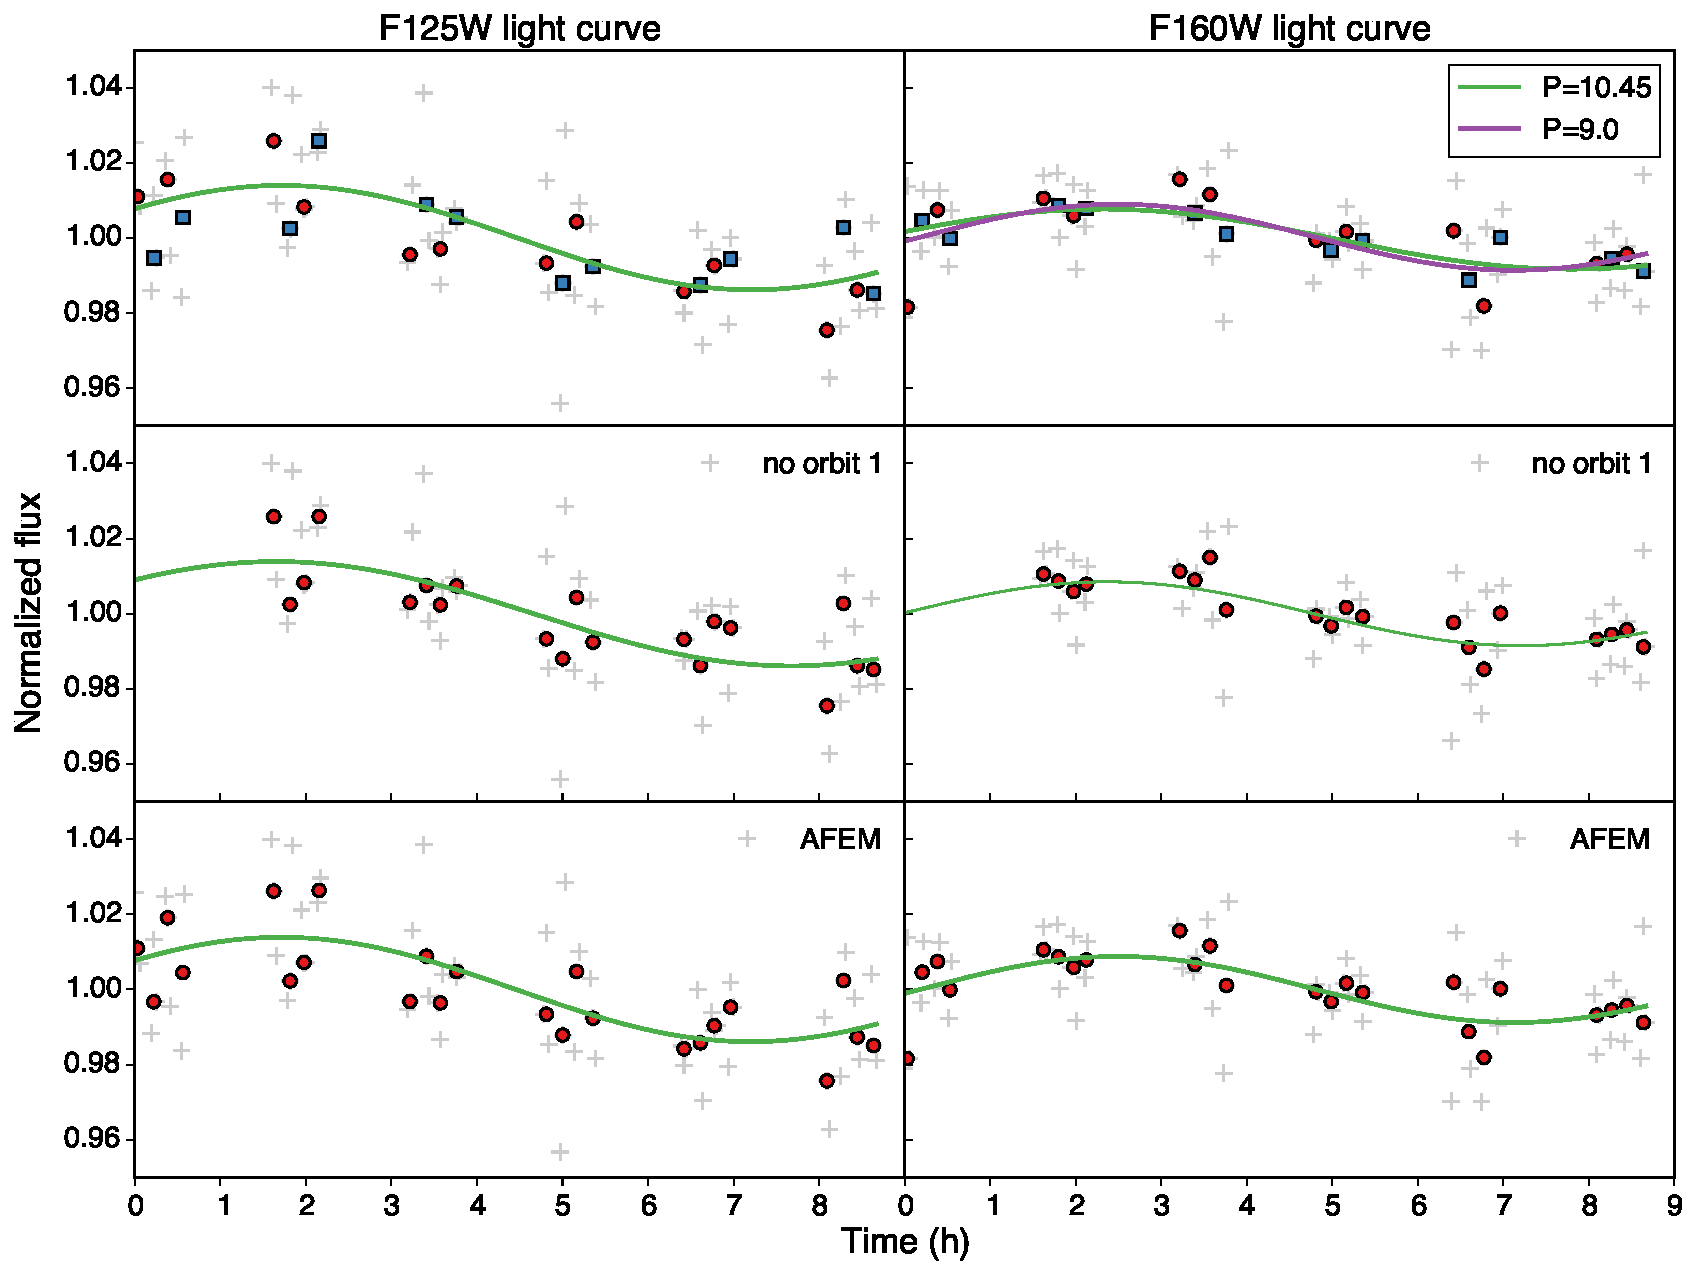
\includegraphics[width=\textwidth]{systematics}
  \caption{Normalized light curves for 2M1207B with filter F125W
    (left) and F160W (right). Original photometric measurements are
    plotted with gray crosses. The two halves of data are binned
    individually, and plotted with red points (first half) and blue
    squares (second half). The F160W light curves are plotted with two
  fitted sinusoidal curves, The green curve is fitted with
  the period fixed to be same as the F125W and the purple curve is
  fitted with all parameter set free.}
  \label{fig:2}
\end{figure*}

\subsection{Tests and Verification}

The light curves that resulted from our photometry show apparently sinusoidal modulations,
discussed in more details in \S,\ref{Results}. To verify that these modulations are intrinsic
to the object and not result of our data reduction procedure or due to instrumental changes, we carried out three different tests. 

First, we fitted sine waves independently to the two filters to verify the similarity of the signal in the two bands. Inconsistent periods or light curve shapes would argue against a genuine signal.
We found that the periods of the best fit sine waves are very similar, 10.9$\pm$XX~h
 for F125W and 9.3$\pm$~h for F160W. These periods are consistent within the uncertainty. Furthermore, these periods are not close to any timescales over which HST or WFC3 are known to changes. 

As a second test we repeated the analysis neglecting the first orbit. The motivation behind this test was that, due to spacecraft thermal settling, the first orbit of HST observations
 is often slightly unstable and is often neglected in high-precision studies (\textbf{citation?}). Indeed, in our analysis 2M1207 A is significantly fainter in the first orbit (Figure \ref{fig:3}) than in the subsequent ones. 
 %The exposure levels at the pixels of the peak of the PSF of 2M1207 B are less than 10,000 e$^{-}$
 %for both two colors, thus image persistence is less of an issue for
 %2M1207 B. 
Our analysis based on orbits 2--6 only found essentially identical results to our analysis of orbits 1--6, based on which we conclude that the first less reliable orbit does not affect our results significantly.

As a third test we explored whether a subset of images, perhaps imperfectly normalized or correlated with specific instrument states, could be driving the light curves into an apparently sinusoidal shape. To test this possibility we split the data into two temporally overlapping halves: sub-dataset one from dithering positions 1 and 3, and sub-dataset two from dithering positions 2 and 4. For both datasets we repeated our analysis independently. 
For both of F125W and F160W, two halves demonstrated similar trend of
 variability as shown in Figure \ref{fig:2}.
 Our analysis detected sinusoidal modulations in {\em both} sub-datasets and in {\em both} filters, with periods and amplitudes consistent with those derived from the complete data set. 
 
 These tests demonstrate that the modulation seen in our data are consistently present in the different filters, in the different time segments of the data, and in data obtained in different dithering positions. 
 % \begin{itemize}
% \item the source of the scattering -- 
% \item flat field uncertainty -- adding artificial flat field error mask
% \item validity of the variability\\
%   -- both filter demonstrate similar period of variability\\
%   -- split the data into two half, the trend in two halves of data
%   looks similar.
%   -- fix the position does not change the light curve
% \item uncertainty of sinusoidal curve fit
%   -- carry out a mcmc fit? is it worth doing this.
% \end{itemize}

\subsection{Amplitude and Period Measurements}

To constrain the uncertainties of the least square optimization
results, we used a Monte Carlo(MC) method to improve the fitting. We
generated a series of random Gaussian noises with the standard deviation same as
the photon noise, added them to the original light curves, and applied
least square fit to the new light curves. We repeated above routine for 10000 times and obtained
the distribution of the fitting parameters. The distributions for the
periods and the amplitudes for F125W and F160W light curves are
shown in Figure \ref{fig:4}.

The distributions for the periods demonstrate long tail shaped towards
long period. The peaks of the two distributions separated by $\sim 1$
hour. The difference of the peaks are within $1-\sigma$. Combing the
measurements from the two light curves, we conclude the rotation period
of 2M1207B to be $9.0_{-1.5}^{+2.5}$ hours.

The variation amplitudes in the two bands have significant
difference. The distributions of the amplitudes are well described by
Gaussian profiles. To fit the histogram to a Gaussian function, we
determined that amplitude distribution of F125W peaks at 1.5\% with a
standard deviation of 0.3\%, and that of F160W have mean and standard
deviation of 0.9\% and 0.2\% correspondingly. The peaks of the two
histograms separated by more than $2-\sigma$. The variation amplitude
of F125W light curve is 1.67 times of that of F160W light curve.

\section{Result}

We present the first high-contrast, high-resolution, high-cadence, and high-precision photometry of a directly imaged planet or planetary-mass companion. Our observations reveal a modulation in the light curve of the 5--7~M$_{J}$ companion 2M1207b, the first detection of modulations in directly imaged ultracool objects.  The best fit periods for F125W and F160W are 10.9 and 9.3 hour correspondingly. The amplitudes for the normalized light curves are 1.4\% and 0.9\% for F125W and F160W light curves. Periods..

We obtained high signal to noise photometry series for both 2M1207 A
and B (Figure \ref{fig:3}). On average, the photometric contrast is $6.52\pm0.03$ for
F125W and $5.77\pm0.02$ for F160W. The difference of F125W contrast
from that measured in J-band \citep{Mohanty2007} and
F160W contrast from that measured with NICMOS F160W 
\citep{Song2006} is due to the different throughput profiles of the
filters.

In the following we will discuss the amplitude and period of 2M1207B and place this object in the broader context of ultracool atmospheres.



\begin{figure*}
  \centering
  \plotone{sineCurveFit_binCombined}
  \caption{Normalized light curves for 2M1207 B (upper) and A (lower)
    with filter F125W (left) and F160W (right). Individual photometric
  measurement are plotted in gray crosses and binned photometry are
  plotted with red points. Best fitted sinusoidal waves are plotted
  with blue solid lines.}
  \label{fig:3}
\end{figure*}


%Although the photometric time series demonstrate relatively large
%scattering, both F125W and F160W light curves demonstrate sinusoidal
%shape with clear temporal variability. We fitted sine waves to the two
%light curves using least square optimization, and determined the
%periods and variation amplitudes.


\begin{figure*}
  \centering
  \plottwo{periodDistr}{amplitudeDistr}
  \caption{Distributions for periods (left) and amplitudes(right) for the light
    curve of F125W and F160W. The bin size for histograms of period is
  0.25 hour and for that of amplitude is 0.5\%. Histograms are
  normalized in the way that total area of the histogram equals to
  1. In the right panel, Gaussian profiles are fitted to the
  histograms and plotted in solid lines.}
  \label{fig:4}
\end{figure*}

\section{Discussion}
Amplitude and Relative Amplitudes: Comparison to other brown dwarfs

Rotation Period: Comparison to Brown Dwarfs and Beta Pic

Method: Opens a new window, successful demonstration, how could it be improved?
Mapping different pressure levels, atmospheric dynamics?

\section{Conclusions}
\begin{itemize}
\item a data-reduction pipeline is developed to obtain high precision
  photometry measurement from high contrast WFC3 IR data. For a
  contrast of $\sim 7$ magnitudes at an angular separation of
  $\sim0.7''$, we obtained photometry measurement for 2M1207 B at
  precision of about 2-3\%. 
\item time variability for 2M1207 B was discovered, the light curve of
  2M1207 B for both two colors can be fitted with a T=10.7 hr
  sinusoidal curve.
\item constrain on the amplitude of the amplitude of the
  variability. Large amplitude can be excluded. Constraints on the
  inhomogeniety of the cloud coverage can be inferred -- small
  thickness variance...
\item ? The atmosphere and cloud structure of 2M1207 B. How does it
  compare to the brown dwarf.
\end{itemize}


\bibliography{ref.bib}
\end{document}

%%% Local Variables:
%%% mode: latex
%%% TeX-master: t
%%% End:
